\chapter{Identification of the LexA binding motif and regulon in the
  Verrucomicrobia}

\section{Introduction}

The global response to DNA damage in Bacteria is known as the SOS response. It
was first described in \textit{Escherichia coli} 40 years ago and has been
observed in a wide range of bacterial species~\citep{radman1975sos,
  little1982sos, erill2007aeons}. In \textit{E. coli} and \textit{Bacillus
  subtilis}, it has been shown to control the expression of up to 40 genes that
are involved in DNA repair, translesion synthesis and cell division
arrest~\citep{au2005genetic, fernandez2000identification, walker2000sos}. The
SOS response is controlled by the transcriptional regulator
LexA~\citep{michel2005after}. Under normal conditions, the LexA binds as a
homodimer to sites upstream of regulated operons, blocking the initiation of
their transcription. When DNA damage occurs, RecA, the other main protein
involved in the SOS response, binds to single-stranded DNA and promotes the
autoproteolysis of the LexA. Self-cleavage of the LexA repressor leads to
de-repression of the SOS response genes, including \textit{lexA} and
\textit{recA}~\citep{little1991mechanism}. In recent years, there has been
growing research interest in the SOS response due to its induction by antibiotic stress
and its involvement in the regulation of mobile genetic elements, such as
integrative-conjugative elements and integron integrase genes~\citep{beaber2004sos,
  guerin2009sos}.

Unlike many transcriptional regulators, the LexA binding motif displays remarkable
divergence across different phyla. LexA has been reported to bind short
inverted repeats (GAAC-N4-GTTC) in the Firmicutes and
Actinobacteria~\citep{au2005genetic, davis2002definition}, large palindromic
motifs (CTGT-N8-ACAG) in the Gammaproteobacteria~\citep{erill2003silico,
  fernandez2000identification} and direct repeat motifs (GTTC-N7-GTTC) in the
Alphaproteobacteria~\citep{erill2004differences,
  fernandez1998identification}. The LexA regulon size and composition also vary
significantly across species. LexA has been reported to regulate from 3 to 40
genes, with a core SOS regulon comprising \textit{lexA}, \textit{recA} and the
mutagenesis operon \textit{imuA-imuB-dnaE2}~\citep{erill2006dispersal}. This
variation in its binding motif and
regulon makes LexA a unique model to study the evolution of transcriptional
regulatory elements.

Verrucomicrobia are a recently established Gram-negative phylum with unusual
wart-like protrusions and eukaryotic-like tubulins~\citep{garrity2001road,
  schlesner2006phylum}. Named after \textit{Verrucomicrobium spinosum}, little
is known about this group of Bacteria. They have recently gained attention due
to their association with eukaryotic hosts, their under-recognized dominance in
soil communities and their significant role in the colonization of the human
gut~\citep{sait2011genomic, bergmann2011under, dubourg2013high}. The
Verrucomicrobia are grouped with the Planctomycetes and the Chlamydiae in the
PVC superphylum which comprises species that are of clinical and
biotechnological interest~\citep{gupta2012molecular}.


The SOS response for the Verrucomicrobia has not been documented but the
representative Verrucomicrobia species, \textit{V. spinosum}, has orthologs for
the three core SOS response genes (\textit{lexA}, \textit{recA} and
\textit{imuA}-\textit{imuB}-\textit{dnaE2} operon), the presence of which
suggests that the Verrucomicrobia have a functional SOS response. This study
documents the \textit{in silico} and \textit{in vitro} characterization of the LexA
binding motif in the Verrucomicrobia and the analysis of the SOS regulatory
network in this phlyum, which is shown to display extreme plasticity in terms of
the size and composition of the regulon.

\section{Results}

\subsection{LexA targets a novel binding motif in the Verrucomicrobia}

The representative Verrucomicrobia species, \textit{V. spinosum} DSM 4136,
possesses the core members of the SOS response, \textit{lexA} (VSP\_RS04780),
\textit{recA} (VSP\_RS32310) and \textit{imuA}-\textit{imuB}-\textit{dnaE2}
(VSP\_RS05590, VSP\_RS05595, VSP\_RS05600), which suggests that the
Verrucomicrobia have a functional LexA regulatory network. A computational
search with known LexA-binding motifs did not detect any putative binding
sites upstream of SOS response related genes in \textit{V. spinosum} which
suggests that \textit{V. spinosum} LexA targets a different motif. The presence
of a novel LexA binding motif in
the Verrucomicrobia was tested by searching for overrepresented patterns in
116 promoter sequences of \textit{V. spinosum} \textit{lexA}, \textit{recA} and
\textit{imuA} orthologs from 59 different assemblies for the Verrucomicrobia
phylum. The most significant motif identified by MEME was a 14 bp palindromic
motif (TGTTC-N4-GAACA), identified in the promoter of 27 \textit{lexA}, 25
\textit{recA} and 3 \textit{imuA} genes of 36 different genome and metagenome
assemblies (Figure~\ref{fig:verruco-lexa}A). A computational search using the
discovered motif identified putative site instances in the promoters of
\textit{V. spinosum} \textit{lexA}, \textit{recA} and \textit{imuA-imuB-dnaE2}
operons (Figure~\ref{fig:verruco-lexa}B).

\begin{figure}
  \centering
  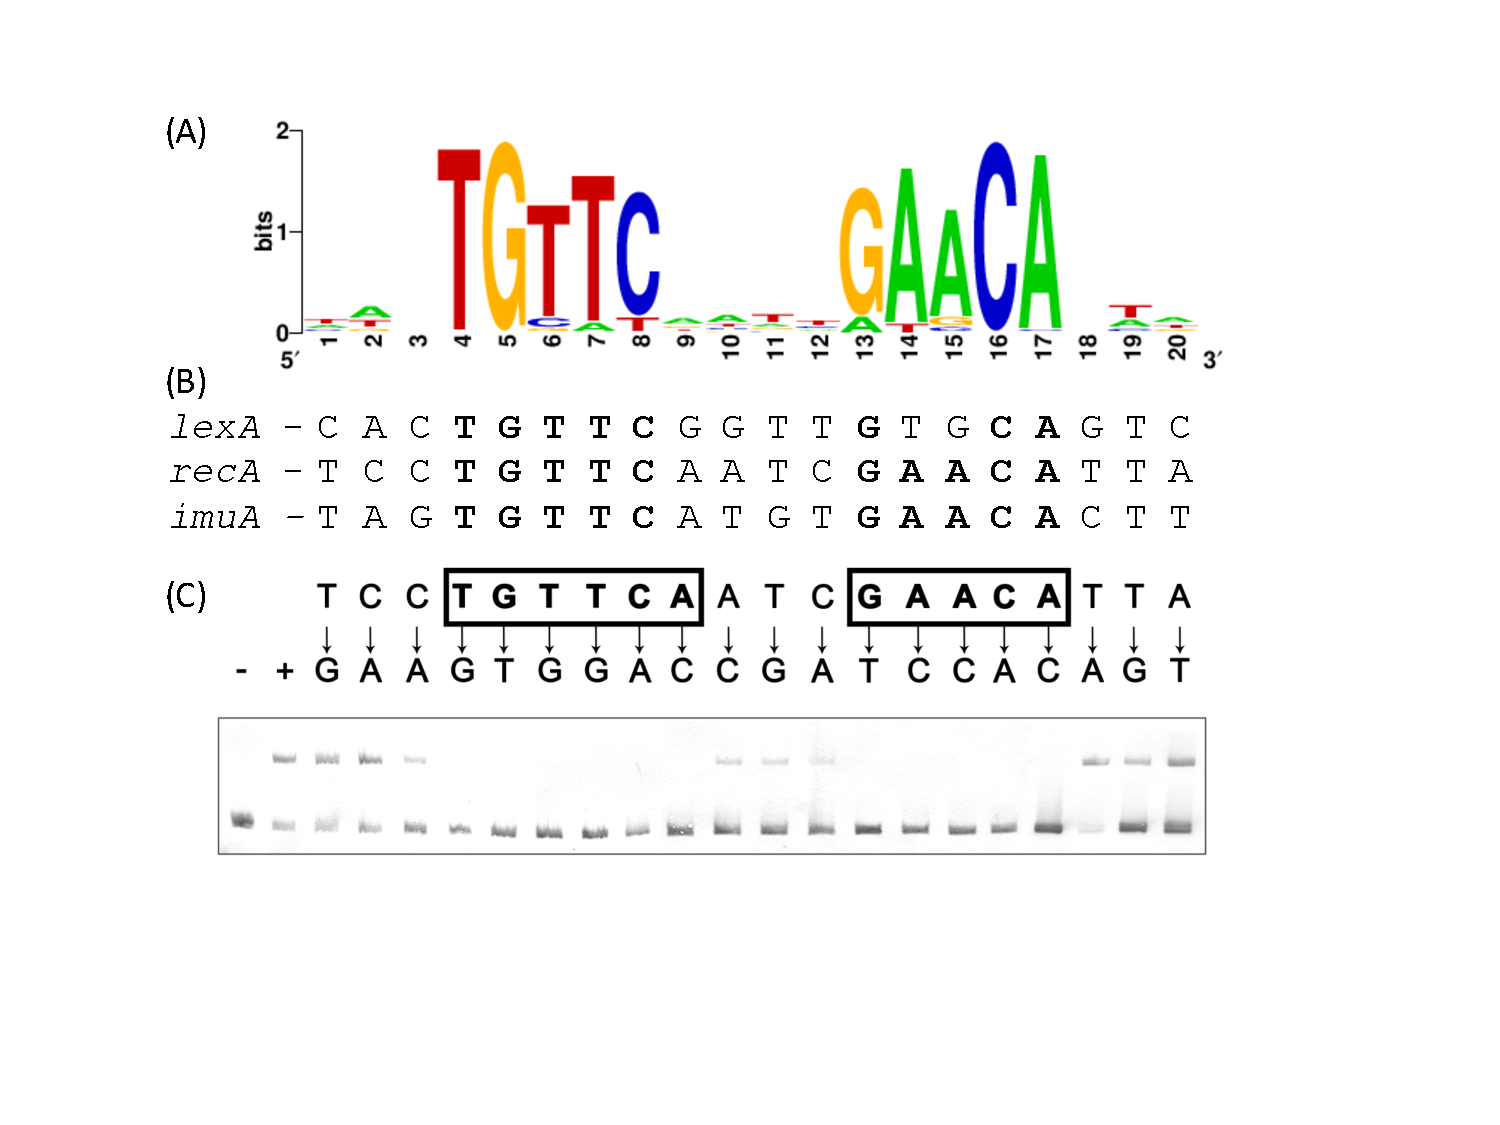
\includegraphics[width=0.7\textwidth]{figures/chapter5/verruco_lexa}
  \caption[(A) Sequence logo of the palindromic LexA motif identified by MEME
  in the promoter regions of Verrucomicrobia \textit{lexA}, \textit{recA} and
  \textit{imuA} genes. (B) The LexA putative binding sites identified in the
  promoter regions of \textit{V. spinosum} \textit{lexA}, \textit{recA} and
  \textit{imuA-imuB-dnaE2} operons.]{(A) Sequence logo of the palindromic LexA
    motif identified by MEME in the promoter regions of Verrucomicrobia
    \textit{lexA}, \textit{recA} and \textit{imuA} genes. (B) The LexA putative
    binding sites identified in the promoter regions of \textit{V. spinosum}
    \textit{lexA}, \textit{recA} and \textit{imuA-imuB-dnaE2} operons. Bases
    matching the consensus sequence are highlighted. (C) Electro-mobility shift
    assays on single-nucleotide mutation containing fragments of the
    \textit{V. spinosum} \textit{recA} promoter using \textit{V. spinosum} LexA
    protein. The ``-'' and ``+'' lanes denote negative control (no LexA
    protein) and positive control (the wild-type \textit{recA} promoter
    fragment), respectively. For all other lanes, the arrows indicate the
    introduced single-nucleotide mutations.}
  \label{fig:verruco-lexa}
\end{figure}

The computationally identified LexA binding motif was experimenally validated
through electro-mobility shift assays (EMSA) and site-directed mutagenesis.
The \textit{V. spinosum} DSM 4136
LexA protein (WP\_009959117) was purified and EMSA was performed with wild-type
and mutants with single nucleotide substitutions at each position of the
predicted binding motif. The results of the site-directed mutagenesis confirm
that LexA binds to a palindromic motif with consensus sequence
TGTTC-N4-GAACA\@. The single-nucleotide mutations to the palindromic regions
(TGTTC and GAACA) eliminate LexA binding to the \textit{recA} promoter,
suggesting that the site is essential for LexA binding
activity~\citep{groban2005binding}. On the other hand, the mutations on the 4 bp
spacer region or 3 bp flanking regions do not alter the binding activity
significantly (Figure~\ref{fig:verruco-lexa}C).

\subsection{The Verrucomicrobia LexA targets tandem sites in \textit{lexA}
  promoters}

A closer look at the \textit{V. spinosum} \textit{lexA} promoter shows that it
contains a poorly conserved LexA binding site 1 bp downstream of the putative
site that was identified \textit{in silico} (Figure~\ref{fig:lexa-tandem}). To
investigate if both of these sites are functional, EMSA was performed with
purified \textit{V. spinosum} LexA protein on the \textit{V. spinosum}
\textit{lexA} promoter. Figure~\ref{fig:emsa1}A shows that low concentration of
LexA protein produces two distinct retardation bands. Increasing the LexA
protein concentration, on the other hand, shows the single band that
corresponds to the occupation of both sites on the \textit{lexA} promoter. The
analysis of \textit{V. spinosum} \textit{lexA} orthologs in the Verrucomicrobia
reveals that many \textit{lexA} promoters display similar tandem configurations
most of which have a conserved TGTTC-N4-GAACA sequence followed by a site where
only the first TGTTC is conserved. (Figure~\ref{fig:lexa-tandem}).

\begin{figure}
  \centering
  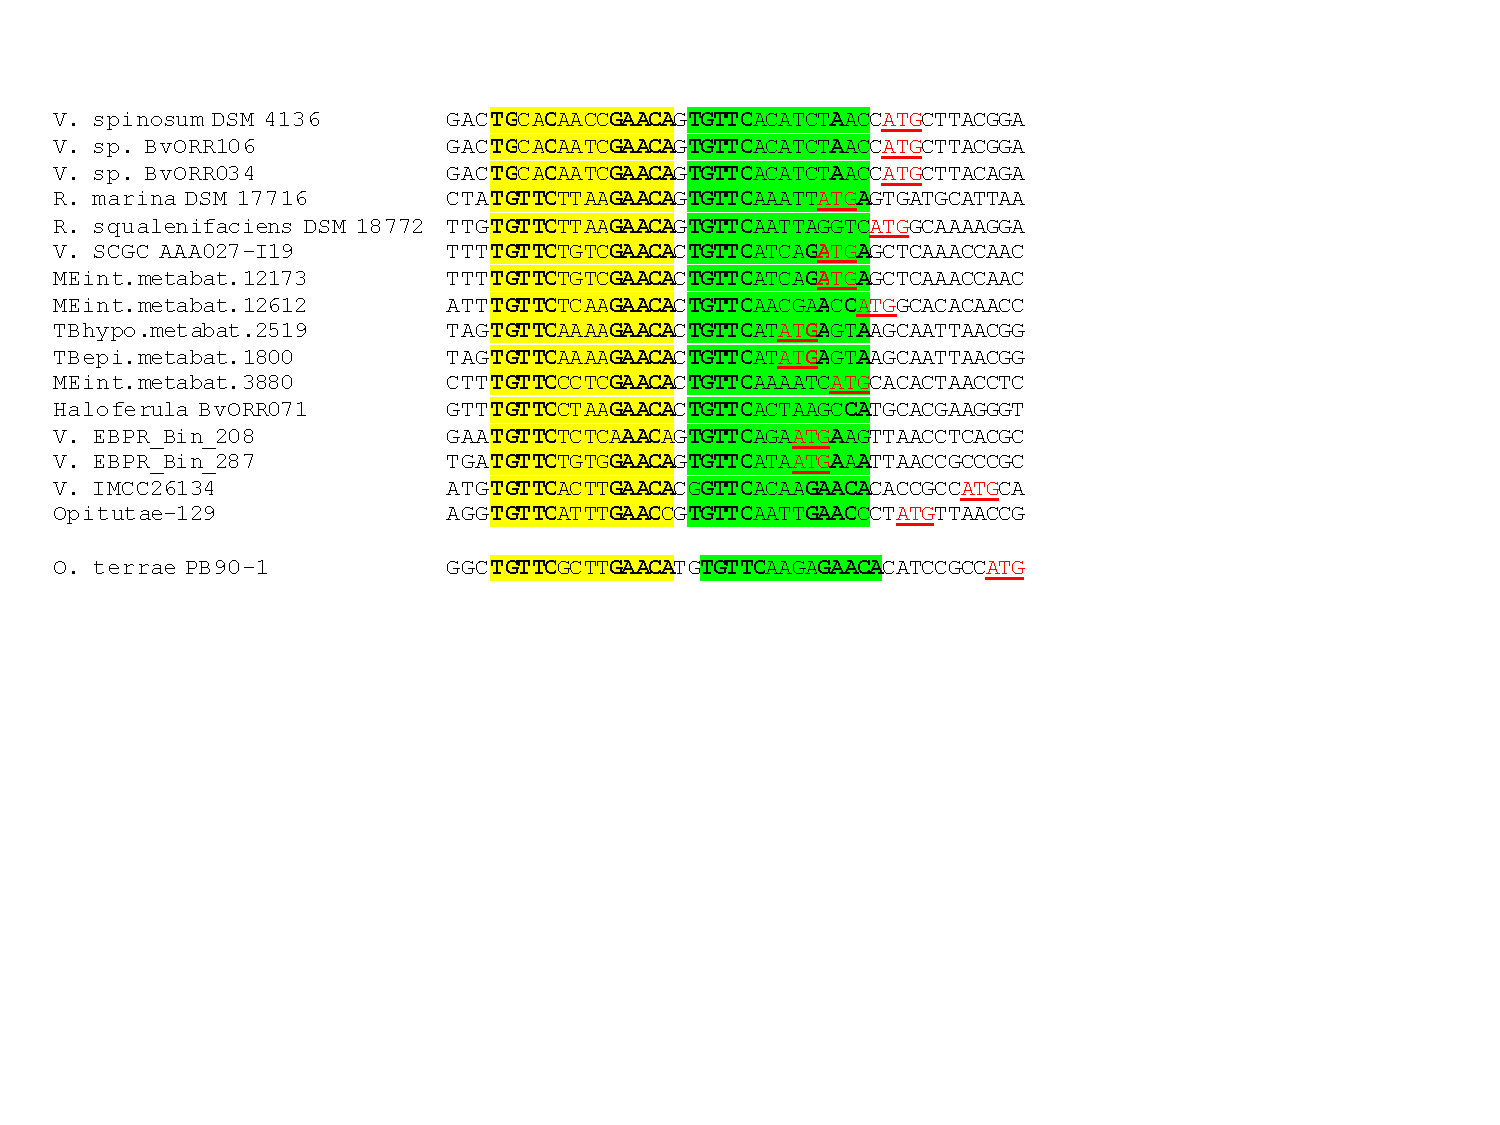
\includegraphics[width=\textwidth]{figures/chapter5/tandem}
  \caption[Multiple sequence alignment of \textit{lexA} promoter sequences in
  Verrucomicrobia.]{Multiple sequence alignment of \textit{lexA} promoter
    sequences in Verrucomicrobia illustrating the tandem LexA binding site
    arrangement observed in \textit{V. spinosum}. The primary and secondary
    LexA binding sites are highlighted in yellow and green, respectively. Bases
    matching the LexA motif consensus sequence are in bold. Predicted
    translation start sites are in red and underlined.}
  \label{fig:lexa-tandem}
\end{figure}

\begin{figure}
  \centering
  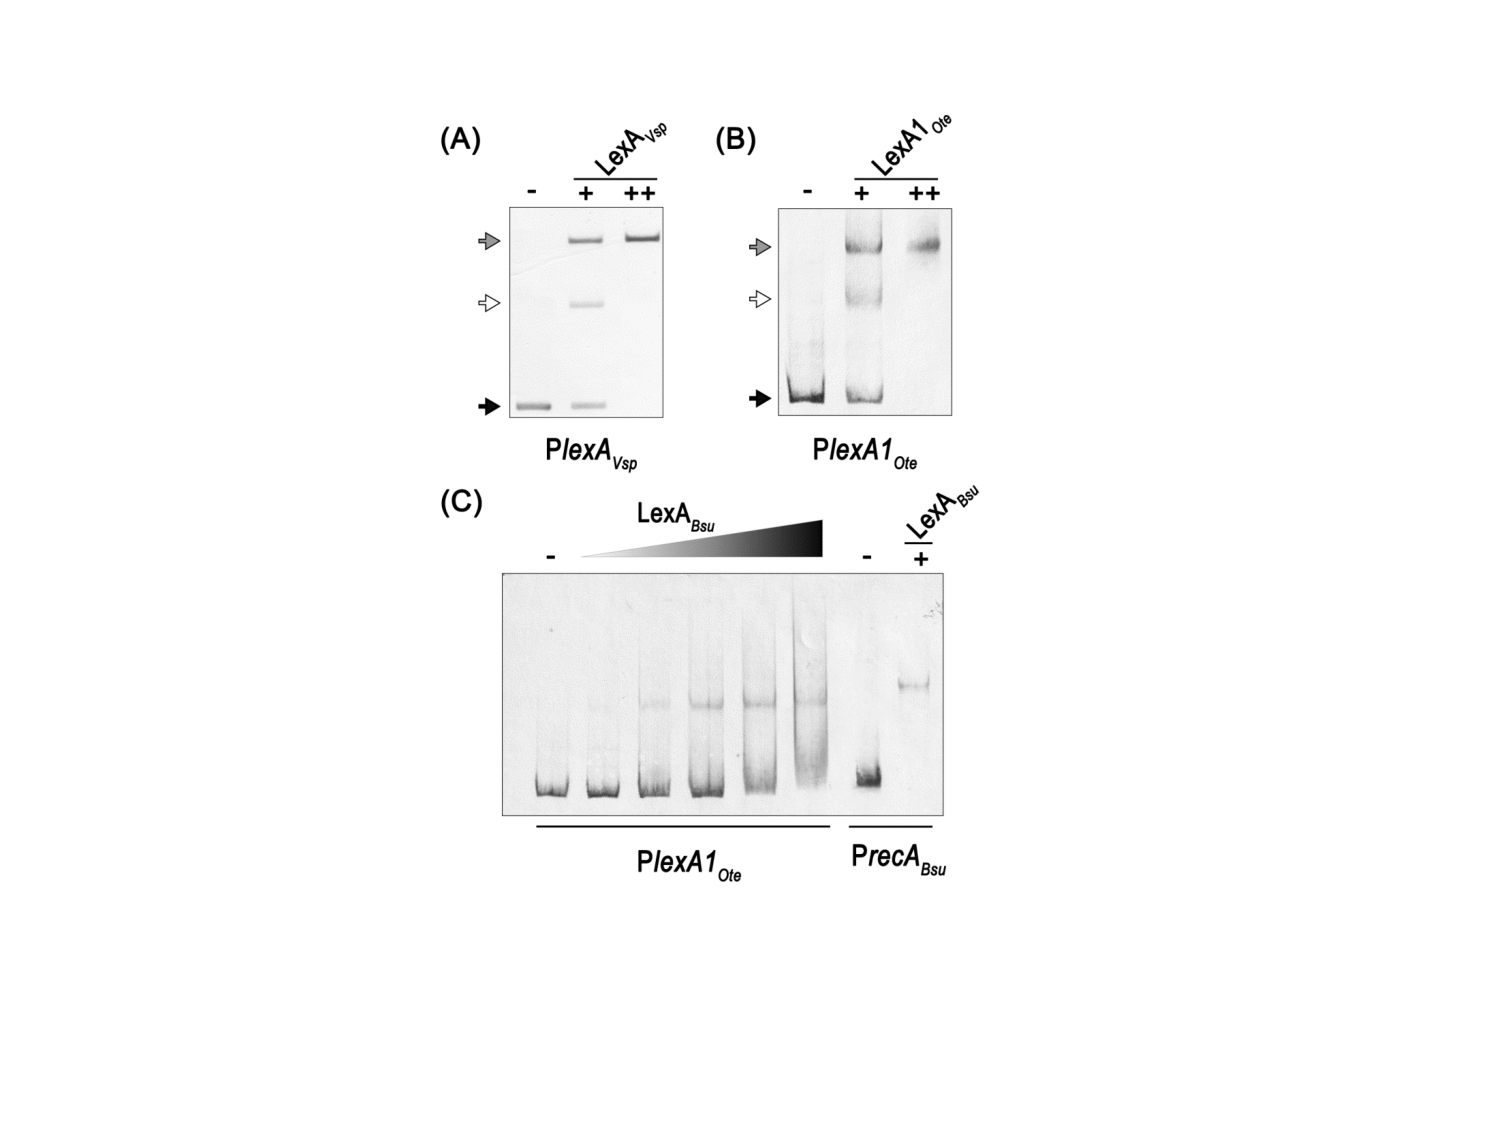
\includegraphics[width=0.5\textwidth]{figures/chapter5/emsa1}
  \caption[Electro-mobility shift assays on Verrucomicrobia \textit{lexA}
  promoters.]{(A) Electro-mobility shift assays on the \textit{V. spinosum}
    \textit{lexA} (VSP\_RS04780) promoter with increasing concentrations of
    \textit{V. spinosum} LexA protein (WP\_009959117). (B) Electro-mobility
    shift assays on the \textit{O. terrae} \textit{lexA} (OTER\_RS20480)
    promoter with increasing concentrations of the \textit{O. terrae} LexA
    protein (WP\_012376858) (C) Electro-mobility shift assays on the
    \textit{O. terrae} (OTER\_RS20480) with increasing concentrations of the
    \textit{B. subtilis} LexA protein (WP\_0032382009). A \textit{B. subtilis}
    \textit{recA} promoter was used as a positive binding control.  In all
    panels, the ``-'', ``+'' and ``++'' denote the absence and addition of 80nM
    and 400nM of protein, respectively. A black arrow indicates unbound DNA, a
    white arrow designates the retardation band due to a single LexA dimer
    binding DNA\@. A grey arrow indicates the retardation band created by two
    LexA dimers binding DNA.}
  \label{fig:emsa1}
\end{figure}


In addition, a member of the Verrucomicrobia phylum, \textit{Opitutus terrae}
PB90-1, has two fully conserved LexA binding motifs in the promoter region of
the putative \textit{lexA-imuA-imuB-dnaE2} operon (OTER\_RS20480,
OTER\_RS20475, OTER\_RS20470, OTER\_RS20465) separated by 2 bp. In this
species, the tandem
arrangement of two LexA-binding sites generates a GAAC-N4-GTTC sequence,
concordant with the LexA binding motif of Firmicutes and Actinobacteria. To
validate the
functionality of this configuration, EMSA with \textit{O. terrae} LexA
(WP\_012376858) was performed revealing two retardation bands at low LexA
protein concentration and confirming that both LexA sites in the
\textit{lexA-imuA-imuB-dnaE2} operon are functional
(Figure~\ref{fig:emsa1}B). EMSA with increasing concentrations of
\textit{B. subtilis} LexA (WP\_0032382009) shows that \textit{B. subtilis} LexA
binds to the motif instance generated by the tandem arrangement in the
\textit{O. terrae} \textit{lexA-imuA-imuB-dnaE2} promoter (Figure~\ref{fig:emsa1}C).

\subsection{The core Verrucomicrobia LexA regulon is composed of three operons
  involved in DNA repair and mutagenesis}

Once the LexA binding motif of the Verrucomicrobia had been identified, a comparative
genomics analysis was performed for the LexA regulon in this phylum. 15
whole-genome shotgun assemblies were compiled for species with a
\textit{V. spinosum} LexA homolog from all three major classes of
Verrucomicrobia (Opitutae, Spartobacteria and Verrucomicrobiae). The
comparative genomics analysis illustrates the presence of a core LexA regulon
that comprises three operons: \textit{lexA}, \textit{recA} and
\textit{imuA-imuB-dnaE2}. A high-scoring binding site is present in
\textit{lexA} promoter of all species except \textit{Verrucomicrobium} sp. 3C,
\textit{Verrucomicrobia bacterium} LP2A and \textit{Pedosphaera parvula}
Ellin514, suggesting that they have a different LexA binding motif. The
\textit{splB} gene appears to be LexA regulated in many \textit{Verrucomicrobiae},
one \textit{Opitutaceae} (\textit{O. terrae}) and \textit{Chthoniobacter
  flavus} Ellin428, the only available assembly of a Spartobacteria. The
\textit{splB} product contains a radical SAM domain (PFAM04055) and homologous
to COG1533 which is classified as a DNA repair photolyase. Several members of
this group have been reported to be regulated by LexA in the Actinobacteria,
the Alphaproteobacteria, the Betaproteobacteria and the
Gammaproteobacteria~\citep{davis2002definition, cirz2006defining,
  sanchez2012analysis, ulrich2013characterization, sanchez2015sos}. Finally,
the species with \textit{splB} regulation also have binding sites upstream of
their \textit{imuA-imuB-dnaE2} operons involved in DNA damage-induced
mutagenesis.

\begin{figure}
  \centering
  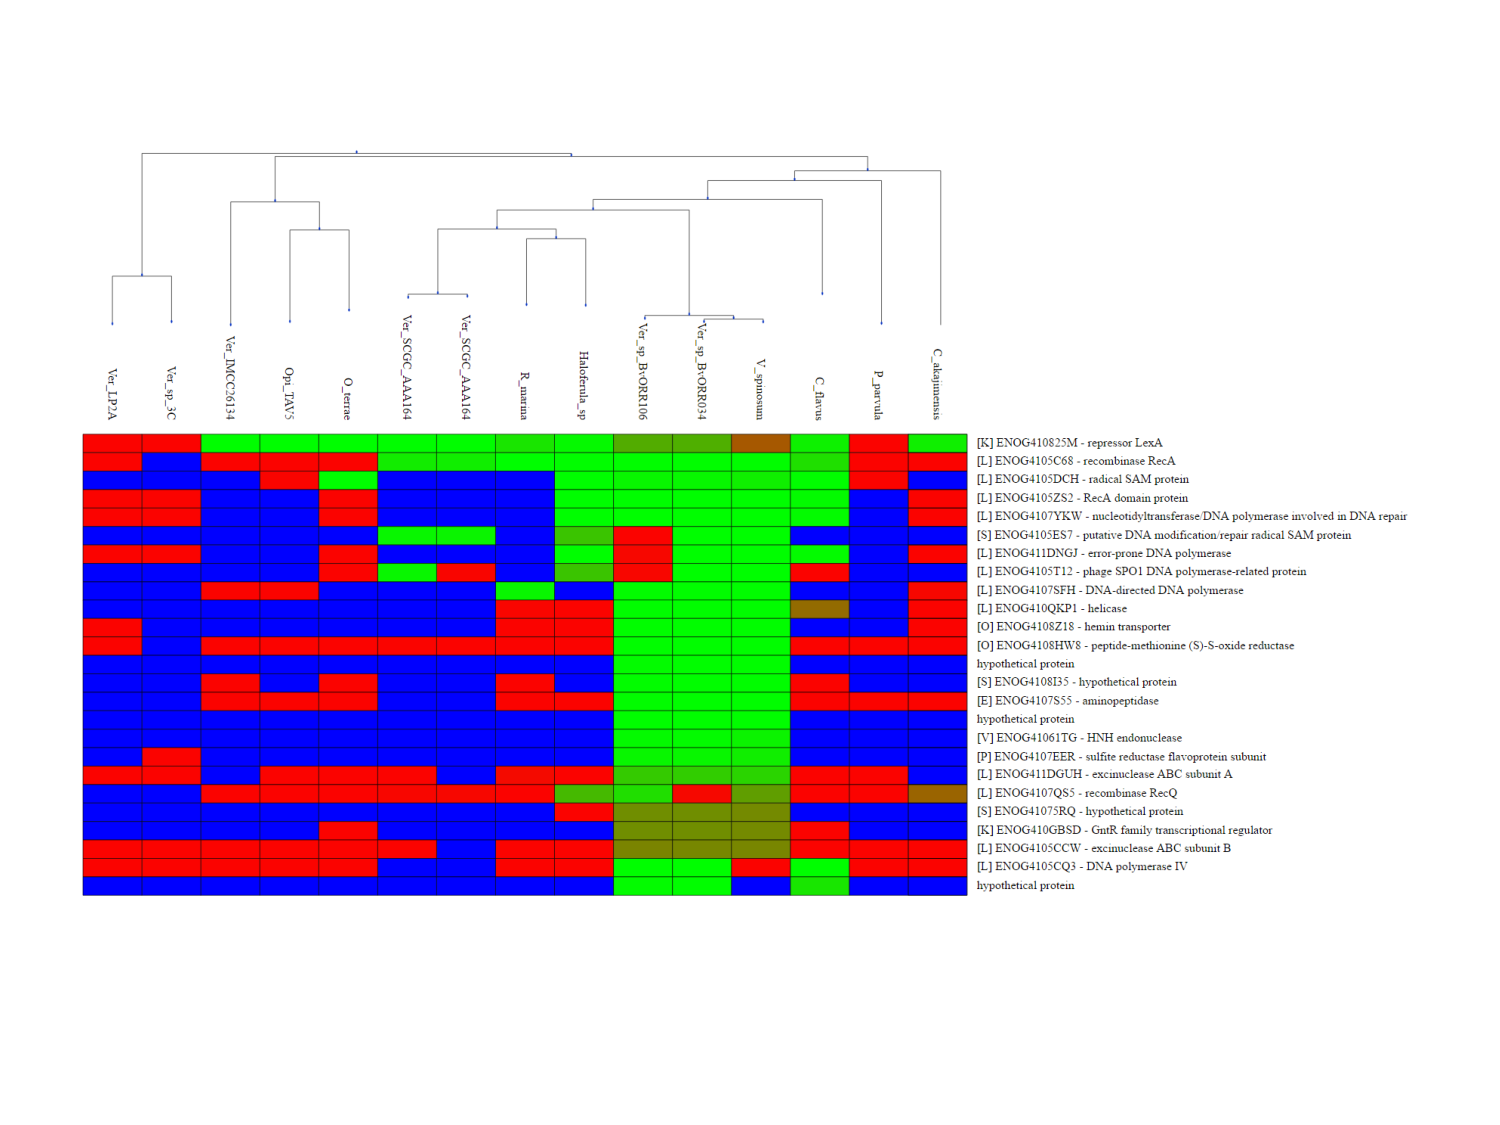
\includegraphics[width=\textwidth]{figures/chapter5/cgb}
  \caption[The comparative genomics results visualized as a heatmap.]{The
    comparative genomics results visualized as a heatmap. Organisms (columns)
    are grouped based on their phylogeny estimated from a LexA protein multiple
    sequence alignment. Each row corresponds to an ortholog group and its
    eggNOG category, identifier and function. The evidence of regulation for
    each species and orthologous group is shown in green-red shades. Light
    green indicates the calculated posterior probability of regulation close to
    one whereas red denotes the probability close to zero. Blue indicates that
    no orthologous gene was identified in a given species.}
  \label{fig:cgb}
\end{figure}

\subsection{The Verrucomicrobia LexA regulon is highly variable and
  incorporates novel functions}

The comparative genomics analysis shows plasticity of the LexA regulon across
the Verrucomicrobia. The predicted regulons range from one operon in
\textit{Verrucomicrobia bacterium} IMCC26134 to 14 operons in
\textit{V. spinosum}. LexA appears to regulate at most two operons in
the \textit{Opitutaceae}. \textit{O. terrae} and \textit{Opitutaceae bacterium}
TAV5 in this family have a duplication of \textit{lexA} gene. The \textit{lexA}
genes in \textit{O. terrae} (OTER\_RS20480) and (OTER\_RS11645) are
significantly diverged (42\% protein sequence identity) and only the promoter
of the \textit{lexA1} gene (OTER\_RS20480) appears to have a functional
Verrucomicrobia LexA-binding
site. In contrast, the \textit{O. bacterium} TAV5 \textit{lexA} genes are 91\%
identical and their promoters contain almost identical LexA binding sites. The
only available Spartobacteria species (\textit{C. flavus}) has a LexA regulon
of intermediate size (5 operons).

For the most part, the composition of the inferred Verrucomicrobia LexA regulon
agrees with the experimental and computational analysis of the SOS response in
other phyla~\citep{erill2007aeons, sanchez2012analysis, sanchez2015sos}. In
addition to the core regulon of \textit{lexA}, \textit{splB} and
\textit{imuA-imuB-dnaE2}, the LexA protein appears to regulate genes coding for
the recombination protein RecA (COG0468), the excinuclease ABC subunit A
(COG0178) and subunit B (COG0556), DNA helicase RecQ (COG0514) and error-prone
DNA polymerase IV (COG0389).

For experimental validation of the comparative genomics analysis, EMSA was
performed with \textit{V. spinosum} and \textit{O. terrae} LexA proteins on
several genes that appear to be regulated. Figure~\ref{fig:emsa2} shows that
LexA binds to the promoter of the \textit{splB} gene in \textit{O. terrae}
(OTER\_RS07185) and \textit{V. spinosum} (VSP\_RS12190). It also shows that
LexA binds to the promoters of the \textit{imuA-imuB-dnaE2} operon, the
\textit{recA} (VSP\_RS04780), \textit{uvrA} (VSP\_RS32650) and the genes coding
for DNA polymerase IV (VSP\_RS08510) and RecQ (VSP\_RS32195). These results
confirm the existence of a core LexA regulon in the Verrucomicrobia phylum.

\begin{figure}
  \centering
  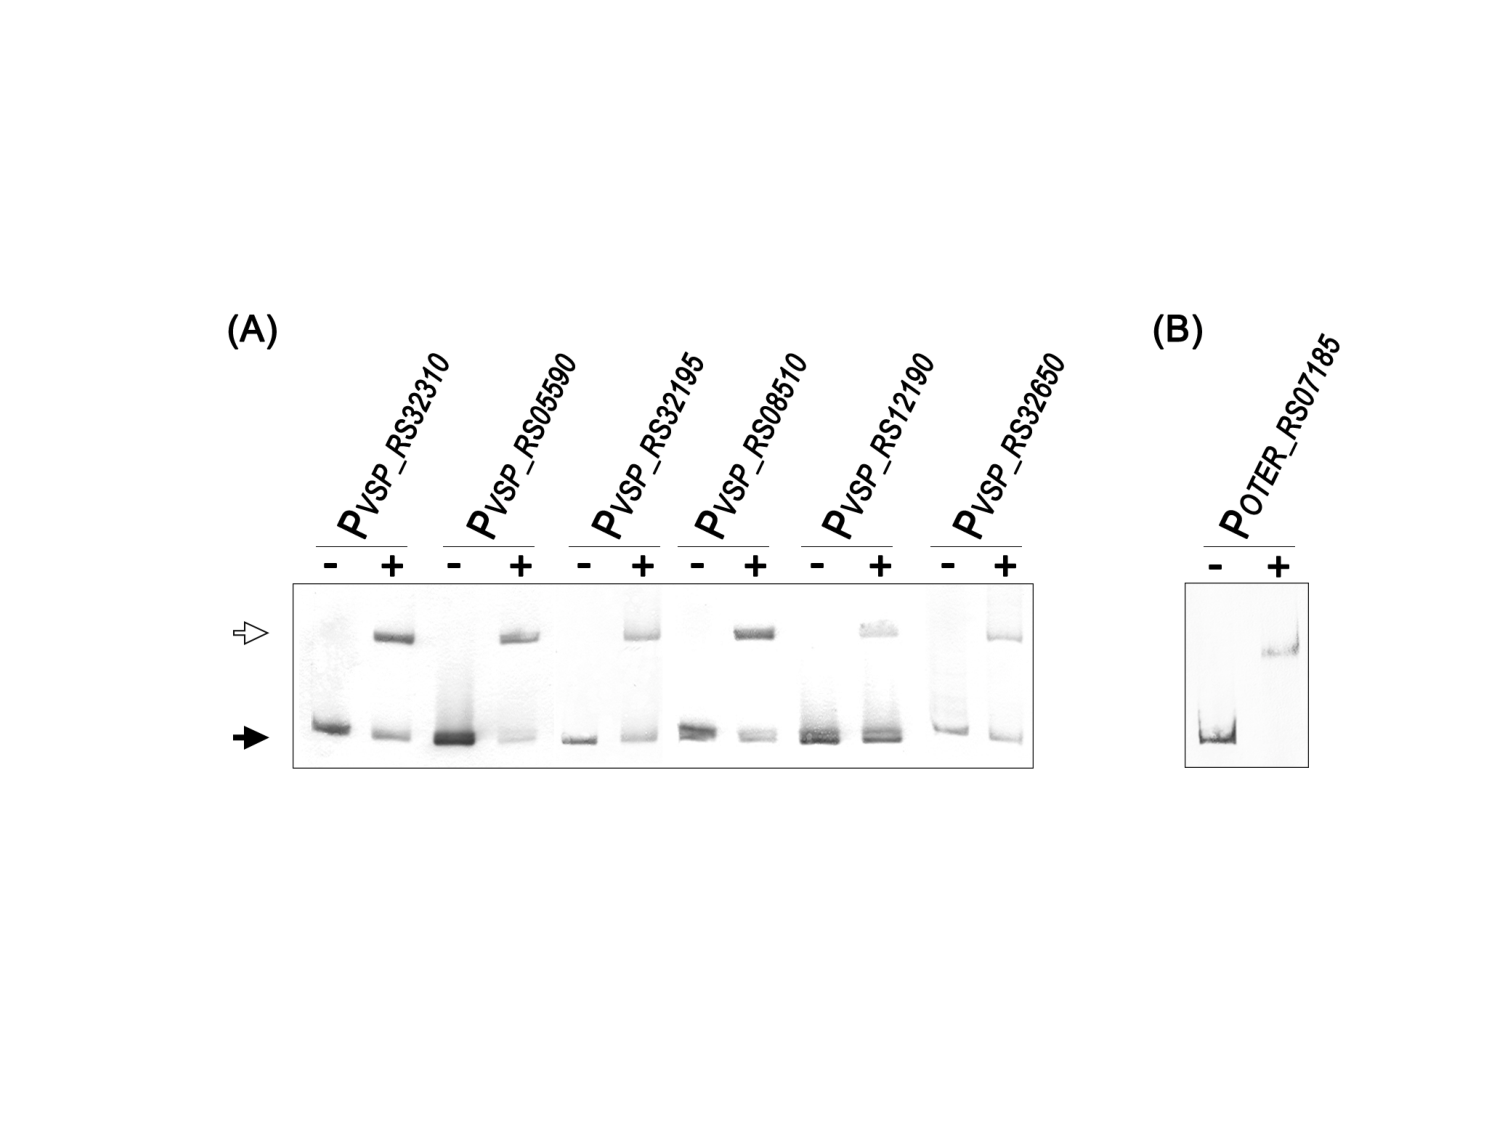
\includegraphics[width=0.7\textwidth]{figures/chapter5/emsa2}
  \caption[Electro-mobility shift assays using LexA protein on the promoter of
  genes predicted to be regulated.]{(A) Electro-mobility shift assays using
    \textit{V. spinosum} LexA protein (WP\_009959117) on the promoter of genes
    predicted to be regulated. (B) Electro-mobility assay using
    \textit{O. terrae} LexA protein (WP\_012376858) on the \textit{O. terrae}
    \textit{splB} (OTER\_RS07185) promoter. In both panels, the ``-'' and ``+''
    symbols denote the absence and presence of the LexA protein,
    respectively. A black arrow indicates unbound DNA and a white arrow
    designates the retardation band due to a single LexA dimer binding DNA\@. }
  \label{fig:emsa2}
\end{figure}

\section{Discussion}

\subsection{Variability and core elements of the SOS regulatory network}
The analysis of LexA regulon in the Verrucomicrobia performed in this work
reveals the presence of a functional LexA protein targeting the same binding
motif in all three major classes, Opitutae, Spartobacteria and Verrucomicrobiae
(Figure~\ref{fig:verruco-lexa}). The conservation of the binding motif across
all three classes suggests that a LexA regulatory network was present in the
ancestor of the Verrucomicrobia. In contrast, the size and composition of the
regulon is highly variable (Figure~\ref{fig:cgb}). Some families such as
the \textit{Methylacidiphilaceae} do not have a LexA homolog, and several species
in the Verrucomicrobiales and Opitutales appear to have a small SOS regulatory
network (1--3 operons). Translesion synthesis polymerases have been
documented to be present as a member of SOS regulatory networks of varying
sizes in many clades~\citep{erill2007aeons, davis2002definition,
  fernandez2000identification, sanchez2015sos, ulrich2013characterization,
  au2005genetic}. The identification of a translesion synthesis operon
(\textit{imuA-imuB-dnaE2}) in the Verrucomicrobia LexA regulon supports the
hypothesis that it was a part of the ancestral SOS response. In addition, the
presence of a photolyase (\textit{splB}) documented in several
clades~\citep{davis2002definition, cirz2006defining, sanchez2012analysis,
  ulrich2013characterization, sanchez2015sos} and its identification as a core
element of the SOS response in the
Verrucomicrobia suggest that photoreactivation might be an essential part of
the primordial SOS response.

Unlike the presence of a translesion synthesis and a putative photolyase, the
SOS response in the Verrucomicrobia differs in many ways from the canonical SOS
regulatory network of \textit{E. coli} and \textit{B. subtilis}. The SOS
regulatory network in the Verrucomicrobia appears to contain RecQ (ENOG4107QS5
and ENOG410QKP1) (Figure~\ref{fig:cgb}) which is involved in the initiation and
the reversal of recombination and reported to cooperate with the SOS genes
\textit{recA} and \textit{ssb}~\citep{heyer2004damage,
  nakayama2005escherichia}. The LexA regulation of RecQ but not other DNA
helicases (uvrD, PcrA, DinG) suggests that RecQ might have a complementary
role in this phylum.

\subsection{A tandem model for the evolution of the LexA binding motif}

Many bacterial transcription factors bind cooperatively to tandem
sites~\citep{barnard2004regulation}. First reported in the \textit{E. coli}
\textit{lexA} promoter~\citep{brent1982regulation}, it has been shown to be a
common feature of \textit{lexA} genes in the Gammaproteobacteria, the
Betaproteobacteria, the Alphaproteobacteria, and the Firmicutes and
Actinobacteria~\citep{sanchez2012analysis, cornish2012inference}. The tandem
sites have also been documented for other SOS genes, such as the \textit{ydjM}
gene of \textit{E. coli}~\citep{fernandez2000identification} or the
\textit{umuDC}-like operon (\textit{yqjW-yqzH}) of
\textit{B. subtilis}\citep{au2005genetic}. This work reports the evidence for a
recent \textit{lexA} duplication in \textit{Opitutaceae} and conservation of
tandem LexA binding sites in the Verrucomicrobia
(Figure~\ref{fig:lexa-tandem}). Mobility assays demonstrating that
Verrucomicrobia LexA binds cooperatively to degenerate sites and that the
tandem configuration generates a functional \textit{B. subtilis} binding site
suggest a novel mechanism for LexA binding motif evolution
(Figure~\ref{fig:emsa1}).

Figure~\ref{fig:model} illustrates the conventional and tandem site-based model
for LexA motif evolution. According to this model, the regulon is under control
of the primary LexA which represses itself via tandem LexA binding sites. Upon
duplication of the \textit{lexA} gene, the secondary \textit{lexA} diverges and
its product LexA protein targets sites created by the tandem site arrangement
which After deletion of the primary \textit{lexA} gene, the secondary LexA is
already in control of the core regulon and can evolve the binding sites on
their promoters by exploiting the half-site affinity.

\begin{figure}
  \centering
  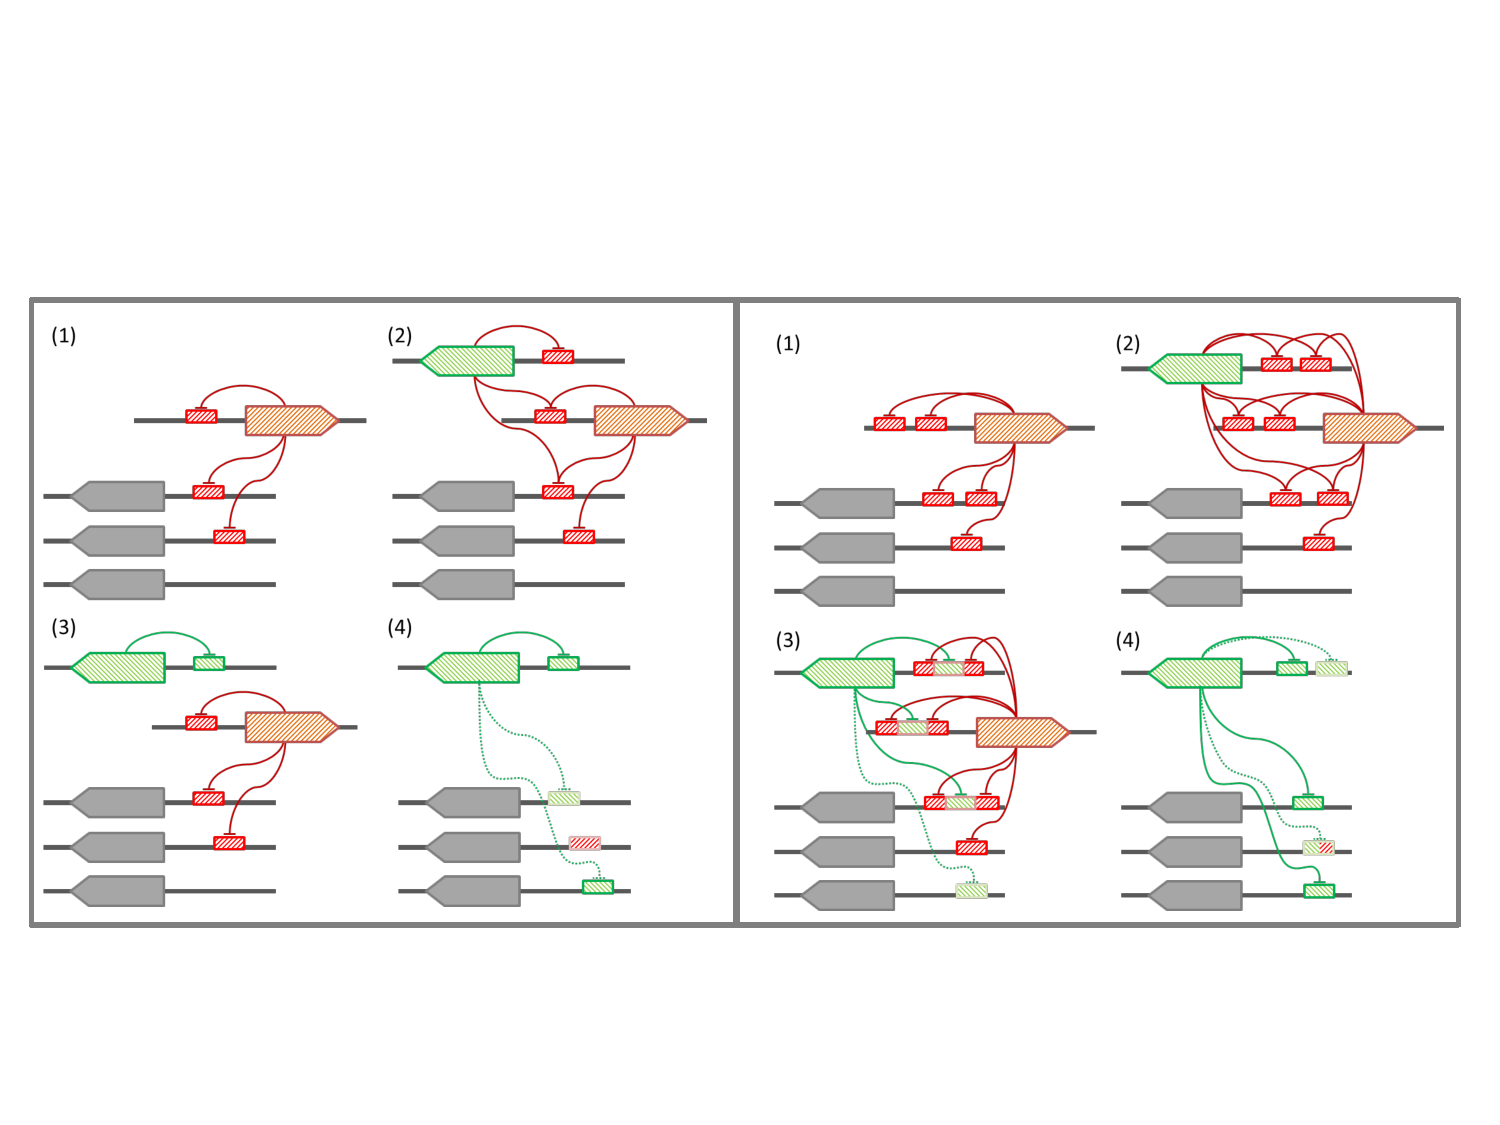
\includegraphics[width=\textwidth]{figures/chapter5/model}
  \caption[Models for evolution of the LexA binding motif.]{(Left panel)
    Conventional model for evolution of the LexA binding motif. (1) Primary
    LexA controls the regulon. (2) A \textit{lexA} gene is duplicated. (3) The
    secondary LexA diverges and targets a novel LexA motif for
    self-regulation. (4) The primary \textit{lexA} gene is deleted and the
    secondary LexA protein takes over the control of the operon due to
    convergent evolution. (Right panel) Tandem site-based model for the motif
    evolution. (1) The primary LexA controls the regulon. It also represses
    itself via tandem LexA binding sites. (2) A \textit{lexA} gene is
    duplicated. (3) The secondary LexA diverges and targets the sites created
    by the tandem site arrangement. (4) The primary \textit{lexA} gene is
    deleted and the secondary LexA protein takes control of the regulon using
    the half-site affinity.}

  \label{fig:model}
\end{figure}

\textit{lexA} duplications targeting identical and divergent motifs have been
experimentally reported as well as their
cross-regulation~\citep{abella2007cohabitation,jara2003geobacter,
  yang2008analyses}. Also, it has been shown that LexA can bind to degenerate
sites that partially match other LexA binding motifs which demonstrates the
possibility of the secondary LexA binding the original and tandem-generated
motifs~\citep{mazon2004lexa}. Firmicutes and Actinobacteria LexA binding motif
has long been assumed to represent the ancestral motif of LexA due to its broad
distribution in several phyla. The mirror image relationship between
Verrucomicrobia and Firmicutes LexA binding motifs and the evidence of
\textit{B. subtilis} LexA binding the site created by the tandem site
arrangement suggest that the Verrucomicrobia LexA binding motif might have
originated after the duplication of a \textit{lexA} gene targeting tandem
arrangement of Firmicutes-like LexA binding sites in a common ancestor of these
lineages.

\section{Materials and Methods}

\subsection{Functional and taxonomical assignments}
The putative function for all reported genes was identified using the HHPRED
web service with default options and e-value threshold of $10^{-30}$ on the
PFAM and COG databases~\citep{soding2005hhpred, finn2015pfam,
  tatusov2000cog}. eggNOG identifiers, categories and descriptions were
retrieved from the eggNOG database, identified for each reported gene using
HMMER~\citep{powell2013eggnog, eddy2011accelerated}. Taxonomy identifiers for
all species were retrieved from the NCBI Taxonomy
server~\citep{federhen2012ncbi}.

\subsection{Ortholog detection and motif discovery}
\textit{V. spinosum} (TaxID: 240016) LexA (WP\_009959117), RecA (WP\_009965965)
and ImuA \mbox{(WP\_009959308)} were retrieved from the NCBI RefSeq
database~\citep{pruitt2007ncbi}. Their orthologs in Verrucomicrobia genome and
metagenome assemblies were downloaded from the Integrated Microbial Genomes
(IMG) after their identification using the Integrated Microbial Genomes (IMG)
BLAST with a $10^{-20}$ e-value threshold~\citep{markowitz2012img,
  altschul1997gapped}. Promoter sequences of the identified orthologs were used
as input for the MEME motif discovery tool, requesting 8-20 bp palindromic
motifs~\citep{bailey2015meme}. The Weblogo sequence service was used to generate
sequence logos~\citep{crooks2004weblogo}.

\subsection{LexA binding motif search and comparative genomics analysis}
Experimentally validated LexA binding motifs were downloaded from the
CollecTF~\citep{kilic2013collectf}. The Verrucomicrobia whole genome shotgun
assemblies were downloaded from the NCBI RefSeq
database~\citep{o2015reference}. xFITOM was used for the LexA binding motif
search on individual genomes~\citep{bhargava2010xfitom}. Comparative genomics
analysis was performed using CGB, described in the previous chapter.

\subsection{\textit{In vitro} validation of LexA-binding sites}

All experimental techniques were performed by Dr. Susana Campoy at the Barbé
laboratory (Universitat Autònoma de Barcelona).

\textit{E. coli} (DH5$\alpha$ and BL21) (Thermo Fisher Scientific) and
\textit{V. spinosum} DSM 4136 strains were grown at 37\textdegree C in
LB~\citep{green264molecular} and at 30\textdegree C in M13 media (DSMZ 607;
German Collection of Microorganisms and Cell Cultures),
respectively. Antibiotics were added to the cultures at reported
concentrations~\citep{green264molecular}.

Plasmid isolation, restriction digestion, DNA ligation, transformation, DNA
extraction and PCR were performed using standard
protocols~\citep{green264molecular}. Restriction enzymes, T4 DNA ligase, DNA
polymerase and the DIG-DNA labeling and detection kit were from Roche
NimbleGen. The oligonucleotides used for this work were purcheased from
Invitrogen. Mutants of the \textit{V. spinosum} \textit{recA} promoter
(VSP\_RS32310) were obtained using oligonucleotides carrying designated
substitutions. The DNA sequence of generated fragments was verified by
sequencing (Macrogen).

\textit{V. spinosum} DSM 4136 DNA was extracted from phosphate buffered (50 mM)
saline (pH 8.0)-washed pellets containing cells using the easy-DNATM DNA
isolation kit (Molecular Probes). The \textit{V. spinosum} DSM 4136 was
amplified using suitable primers and cloned into a pET15b vector
(Millipore). The \textit{O. terrae} PB90-1 \textit{lexA} was obtained by
chemical synthesis (GeneArt; Thermo Fisher Scientific) and cloned into a pET15b
vector. Overexpression and purification of the \textit{V. spinosum} DSM 4136
and \textit{O. terrae} PB90-1 and \textit{B. subtilis} LexA proteins was
performed as described previously for other LexA
proteins~\citep{cambray2011prevalence, cornish2014characterization}. DNA probes
for electro-mobility shift assays were generated using two complementary
synthetic oligonucleotides centered on the target LexA-binding sites.The dsDNA
synthetic fragments were ligated into pGEMT vector (Roche NimbleGen) and
transformed into \textit{E. coli} DH5$\alpha$ (Thermo Fisher Scientific). In
all cases the plasmids were confirmed by sequencing and DNA probes were
obtained by PCR using M13 forward and reverse digoxigenin-labelled
oligos. EMSAs were performed as described
previously~\citep{sanchez2012analysis}, using 20 ng of each digoxigenin-marked
DNA probe in the binding mixture and adding the corresponding LexA protein
(from 80 to 400 nM). Samples were loaded onto 6\% non-denaturing Tris-glycine
polyacrylamide gels and digoxigenin-labeled DNA-protein complexes were detected
using the manufacturer's protocol (Roche NimbleGen).



\section{Conclusion}
This study describes a novel LexA binding motif in the Verrucomicrobia phylum
with a combination of \textit{in silico} and \textit{in vitro} methods. Site
directed mutagenesis of the \textit{V. spinosum} \textit{recA} promoter
confirms that LexA binds a 14 bp palindromic motif with consensus sequence
TGTTC-N4-GAACA. The comparative genomics analysis identifies the core
components of the SOS response and reveals that the LexA regulon varies
significantly in its size and composition across the Verrucomicrobia. The
identification of tandem LexA binding sites generating instances of other LexA
binding motifs allows postulating a novel mechanism of LexA binding motif
evolution.
